\begin{frame}{3.4 보--기둥 접합부}
\textbf{3.4.1 일반사항}
\begin{enumerate}
	\item[(1)] 본 절에서는 보--기둥 접합부 완전강접모멘트접합부 형식만을 고려하며 아래의 접합부를 대상으로 한다. 
	\begin{enumerate}[label=\large\protect\textcircled{\small\arabic*}]
		\item 용접비보강플랜지 (Welded Unreinforced Flange, WUF)
		\item 보플랜지절취형 (Reduced Beam Section, RBS)
		\item 용접하부헌치 (Welded Bottom Haunch)
		\item 용접보강판 (Welded Cover Plate)
	\end{enumerate}	
	\item[(2)] 접합부를 보강하거나 보의 단면을 약화시켜 소성힌지의 위치를 보 내부로 위치시키는 경우, 이를 감안하여 접합부를 모델링한다. 
\end{enumerate}

\begin{block}{ASCE 41-17 9.4.2 FR Moment Frames}
	Moment frames with connections shall be defined as FR if the joint deformations (not including PZ deformation) do not contribute more than 10\% \texttt{(c.f. during the elastic range of response, AISC 342 Draft)} to the total lateral deflection of the frame and the connection is at least as strong as the weaker of the two members being joined. 
\end{block}
\end{frame}


\begin{frame}{3.4 보--기둥 접합부}

	\textbf{3.4.2 보--기둥 접합부의 강성}

\begin{enumerate}
	\item[(1)] 보--기둥 접합부의 강성은 구조역학 원칙에 기반하여 $\ulcorner$건축물 강구조 설계기준 (KDS 41 31 00:2019)$\lrcorner$에 따라 산정한다. 
	\item[(2)] 보--기둥 접합부의 회전강성은 접합부를 보강하거나 보의 단면을 약화시켜 소성힌지의 위치를 보 내부로 위치시키는 경우가 아닌 한 반드시 모델링 할 필요는 없다. 이러한 경우 보의 유효스팬을 구현하기 위해 접합부를 강체로 모델링한다. 
\end{enumerate}

\end{frame}

\begin{frame}{3.4 보--기둥 접합부}

	\textbf{3.4.3 보--기둥 접합부의 강도}

3.4.3.1 선형동적절차

접합부의 모든 강도는 모든 잠재적 파괴모드를 고려하여 산정한다. 

3.4.3.2 비선형정적 및 동적절차

\begin{enumerate}
	\item[(1)] 비선형정적절차의 경우 표 3-1에 따라 그림 1-1과 같은 비선형 부재력--변형 관계를 결정한다. 보--기둥 접합부의 예상부재강도 $Q_{CE}$는 선형절차와 동일한 값을 사용한다. 
	\item[(2)] 비선형동적절차의 이력거동 모델링은 실험이나 정밀해석을 통해 얻어진 관계를 사용할 수 있으며, 포락곡선으로는 표 3-6에 사용된 모델을 적용할 수 있다. 
\end{enumerate}
\end{frame}	



\begin{frame}
	\begin{figure}
		\centering
		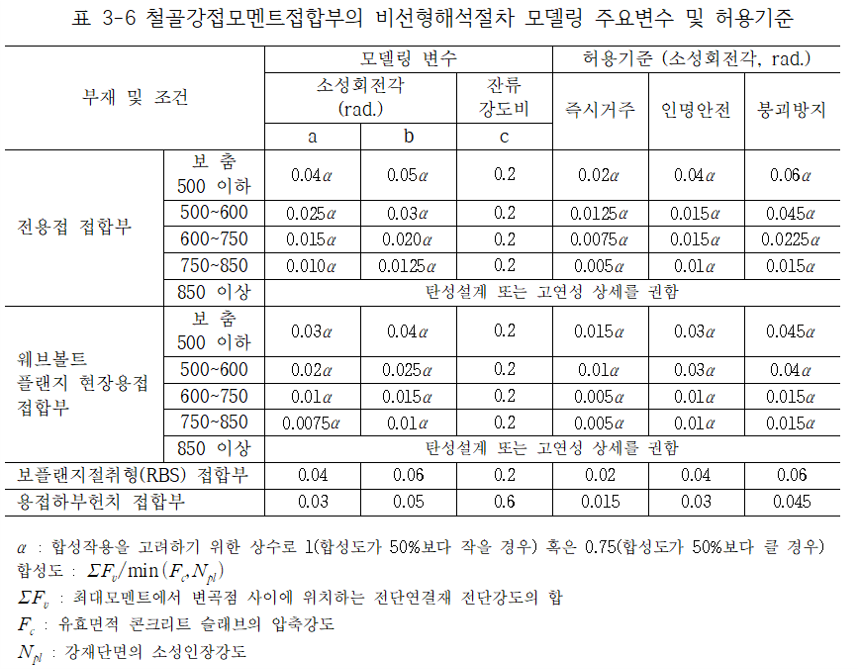
\includegraphics[width=.99\textwidth]{table3-6}
	\end{figure}
\end{frame}	




	\begin{frame}{3.4 보--기둥 접합부}

	\textbf{3.4.4 보--기둥 접합부의 허용기준}

3.4.4.1 일반사항

보--기둥 접합부는 변형지배거동으로 분류한다. 

3.4.4.2 선형동적절차

\begin{enumerate}
	\item[(1)] 보--기둥 접합부의 허용조건은 연속판의 상세, 보 순경간 길이--깊이 비, 보의 웨브와 플랜지의 폭--두께비 등의 조건을 고려하여 표 3-5에 의한 $m$계수를 다음과 같이 수정한다. 각 조건에 의한 수정은 모두 누가하여 산정하나 $m$계수가 1.0 이하일 필요는 없다. 
	\item[(2)] 연속판(Continuity plates)상세: 다음 중 하나 이상의 조건을 만족하지 못할 경우 표 3-5에 의한 $m$계수 값에 0.8을 곱한다. 
			\[t_{cf} \geq \frac{b_{bf}}{5.2}\]
			\[\frac{b_{bf}}{7}<t_{cf}<\frac{b_{bf}}{5.2}~\mathrm{and}~t\geq\frac{t_{bf}}{2}\]
			\[t_{cf}<\frac{b_{bf}}{7}~\mathrm{and}~t\geq\frac{t_{bf}}{2}\]
\end{enumerate}

	\end{frame}
	
	
	\begin{frame}{3.4 보--기둥 접합부}

	\textbf{3.4.4 보--기둥 접합부의 허용기준}

3.4.4.2 선형동적절차

\begin{enumerate}
	\item[(3)] 보 순경간길이--깊이 비: 보의 순경간길이--깊이 비 $L_c/d$가 10보다 클 경우, 표 3-5에 의한 $m$계수의 값에 $1.4-0.04(L_c/d)$를 곱한다. 
	\item[(4)] 보 플랜지 및 웨브의 폭--두께비
	\begin{enumerate}[label=\large\protect\textcircled{\small\arabic*}]
		\item 보 플랜지 및 웨브의 폭--두께비가 다음 조건을 모두 만족할 경우, 표 3-5에 의한 $m$계수의 값은 수정하지 않고 사용할 수 있다. 
		\[\frac{b}{t_f}\leq 0.3\sqrt{\frac{E}{F_{ye}}},~\frac{h}{t_w}\leq 2.46\sqrt{\frac{E}{F_{ye}}}\]
		\item 보 플랜지 혹은 웨브의 폭--두께비가 다음 조건의 한계치를 초과할 경우 표 3-5에 의한 $m$계수의 값에 0.5를 곱하여 사용한다. 
		\[\frac{b}{t_f}> 0.38\sqrt{\frac{E}{F_{ye}}},~\frac{h}{t_w}> 3.76\sqrt{\frac{E}{F_{ye}}}\]		
		\item 두 수식 사이의 값일 경우 수정계수는 직선보간을 통해 구하고 (...이하 생략)
	\end{enumerate}		
\end{enumerate}

	\end{frame}	
	

	\begin{frame}
	\begin{figure}
		\centering
		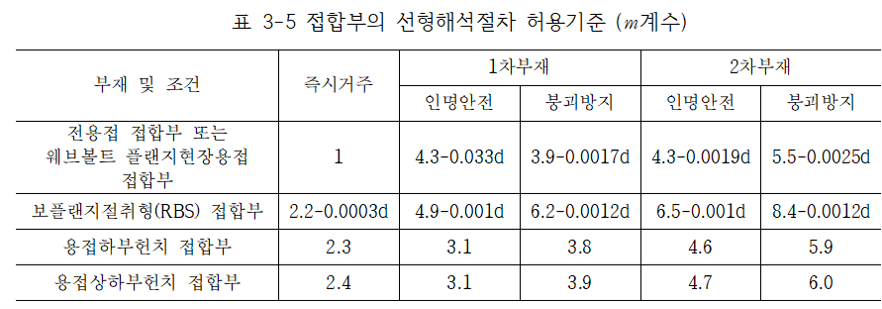
\includegraphics[width=.99\textwidth]{table3-5}
	\end{figure}
\end{frame}



	\begin{frame}{3.4 보--기둥 접합부}

	\textbf{3.4.4 보--기둥 접합부의 허용기준}

3.4.4.3 비선형 정적 및 동적절차

보--기둥 접합부의 허용조건은 연속판의 상세, 보 순경간 길이--깊이 비, 보의 웨브와 플랜지의 폭--두께비 등의 조건을 고려하여 표 3-6에 의한
허용기준을 다음과 같이 수정한다. 각 조건에 의한 수정은 모두 누가하여 산정한다. 

\begin{enumerate}
	\item[(1)] 연속판(Continuity plates)상세: 다음 중 하나 이상의 조건을 만족하지 못할 경우 표 3-6에 의한 허용소성회전각에 0.8을 곱한다. 
			\[t_{cf} \geq \frac{b_{bf}}{5.2}\]
			\[\frac{b_{bf}}{7}<t_{cf}<\frac{b_{bf}}{5.2}~\mathrm{and}~t\geq\frac{t_{bf}}{2}\]
			\[t_{cf}<\frac{b_{bf}}{7}~\mathrm{and}~t\geq\frac{t_{bf}}{2}\]
	\item[(2)] 보 순경간길이--깊이 비: 보의 순경간길이--깊이 비 $L_c/d$가 10보다 클 경우, 표 3-6에 의한 허용소성회전각에 $0.5^{[(8-L_c/d)/3]}$을 곱한다. 
	\item[(3)] 보 플랜지 및 웨브의 폭-두께비 (이하 생략)
\end{enumerate}
	\end{frame}	
	
	
	
\begin{frame}
	\begin{figure}
		\centering
		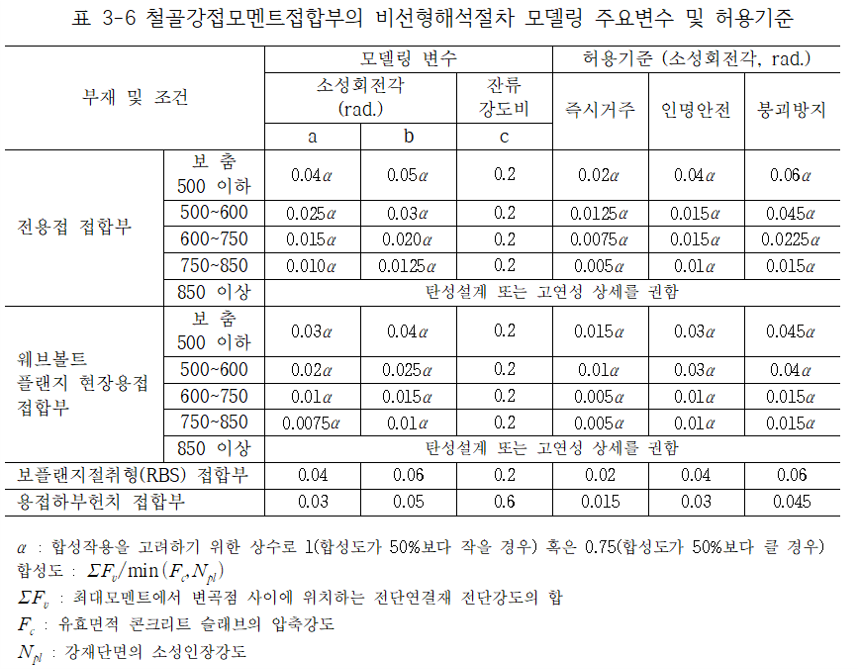
\includegraphics[width=.99\textwidth]{table3-6}
	\end{figure}
\end{frame}	
